% all-in-one cheatsheet layout (Michael Franzen, 2013)
\documentclass[a4paper]{article}

% geometry settings
\usepackage[top=2cm, bottom=2.5cm, left=2cm, right=2cm]{geometry}

% font settings
%\usepackage[light,math]{kurier}
\usepackage[T1]{fontenc}
\usepackage[utf8]{inputenc}
\usepackage{marvosym}
\usepackage{amssymb}
\usepackage{amsfonts}
\usepackage{amsmath}
\usepackage{amsthm}

% colors
\usepackage{xcolor}
\definecolor{lightgray}{gray}{0.8}

% formatting
\usepackage{paralist}
\usepackage{multicol}
\usepackage{tabularx}
\usepackage{Tabbing}
\usepackage{booktabs}
\usepackage{fancyhdr}
\usepackage{url}
\usepackage{mdframed}
\pagestyle{fancy}

% math
\usepackage{array}
\usepackage{eqnarray}
\usepackage{mathtools}

% figures
\usepackage{wrapfig}
\usepackage{subfig}

% figure modules
\usepackage{graphicx}
\usepackage{tikz}
\usetikzlibrary{positioning,calc, shapes}
\usepackage{algorithm2e}
\usepackage{verbatim}

% TOC & Glossary
\usepackage{sectsty}
\usepackage[nottoc,notlof,notlot]{tocbibind}
\usepackage[titles,subfigure]{tocloft}

% commands
\usepackage{xargs}
\usepackage{ifthen}

% head line
\fancyhf{}
\chead{Graph Theory - Sheet 2 - \today\\J. Batzill (1698622), M. Franzen (1696933), J. Labeit (1656460)}
\renewcommand{\headrulewidth}{0.4pt} %obere Trennlinie

\newcommand{\sheetnumber}{1}

% (problem number)
\surroundwithmdframed[
    hidealllines=true,
    backgroundcolor=gray!10,
    skipbelow=\baselineskip,
    skipabove=\baselineskip
]{mylemma}

\surroundwithmdframed[
	linecolor=white,
	skipbelow=\baselineskip,
	skipabove=\baselineskip
]{mytheorem}

\begin{document}
	
	\newtheorem{mytheorem}{Theorem}[section]
	\newtheorem{mylemma}{Lemma}[mytheorem]	

	\newenvironmentx*{solution}[1]{\section*{Problem #1}\addtocounter{section}{1}\setcounter{mylemma}{0}\setcounter{mytheorem}{0}}{}
	\newenvironmentx*{theorem}[1]{\begin{mytheorem}#1\begin{proof}}{\end{proof}\end{mytheorem}}
	\newenvironmentx*{lemma}[1]{\begin{mylemma}#1\begin{proof}}{\end{proof}\end{mylemma}}


	\begin{solution}{5}
		\begin{center}
			
			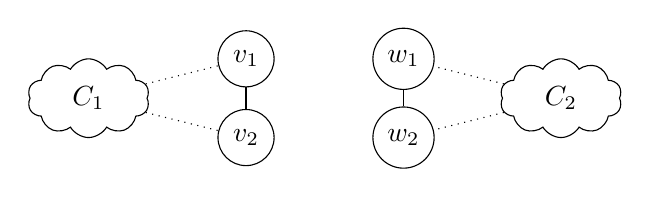
\begin{tikzpicture}
				\node[cloud, cloud puffs=10, cloud puff arc=120, aspect=2, minimum width=1.5cm, minimum height=1cm, draw] (c1)  at (-1,-0.5) {$C_1$};
				\node[circle, draw] (v1) at (1, 0) {$v_1$};
				\node[circle, draw] (v2) at (1, -1) {$v_2$};
				\draw[dotted] (c1) -- (v1);
				\draw[dotted] (c1) -- (v2);
				\draw (v1) -- (v2);

				\node[cloud, cloud puffs=10, cloud puff arc=120, aspect=2, minimum width=1.5cm, minimum height=1cm, draw] (c2)  at (5,-0.5) {$C_2$};
				\node[circle, draw] (w1) at (3, 0) {$w_1$};
				\node[circle, draw] (w2) at (3, -1) {$w_2$};
				\draw[dotted] (c2) -- (w1);
				\draw[dotted] (c2) -- (w2);
				\draw (w1) -- (w2);
			\end{tikzpicture}
		\end{center}
		\textbf{Step 1:}
		\begin{center}
			\begin{tikzpicture}
				\node[cloud, cloud puffs=10, cloud puff arc=120, aspect=2, minimum width=1.5cm, minimum height=1cm, draw] (c1)  at (-1,-0.5) {$C_1$};
				\node[circle, draw] (v1) at (1, 0) {$v_1$};
				\node[circle, draw] (v2) at (1, -1) {$v_2$};
				\draw[dotted] (c1) -- (v1);
				\draw[dotted] (c1) -- (v2);
				\draw (v1) -- (w1);

				\node[cloud, cloud puffs=10, cloud puff arc=120, aspect=2, minimum width=1.5cm, minimum height=1cm, draw] (c2)  at (5,-0.5) {$C_2$};
				\node[circle, draw] (w1) at (3, 0) {$w_1$};
				\node[circle, draw] (w2) at (3, -1) {$w_2$};
				\draw[dotted] (c2) -- (w1);
				\draw[dotted] (c2) -- (w2);
				\draw (w1) -- (w2);
			\end{tikzpicture}
		\end{center}
		\textbf{Step 2:}
		\begin{center}
			\begin{tikzpicture}
				\node[cloud, cloud puffs=10, cloud puff arc=120, aspect=2, minimum width=1.5cm, minimum height=1cm, draw] (c1)  at (-1,-0.5) {$C_1$};
				\node[circle, draw] (v1) at (1, 0) {$v_1$};
				\node[circle, draw] (v2) at (1, -1) {$v_2$};
				\draw[dotted] (c1) -- (v1);
				\draw[dotted] (c1) -- (v2);
				\draw (v1) -- (w1);

				\node[cloud, cloud puffs=10, cloud puff arc=120, aspect=2, minimum width=1.5cm, minimum height=1cm, draw] (c2)  at (5,-0.5) {$C_2$};
				\node[circle, draw] (w1) at (3, 0) {$w_1$};
				\node[circle, draw] (w2) at (3, -1) {$w_2$};
				\draw[dotted] (c2) -- (w1);
				\draw[dotted] (c2) -- (w2);
				\draw (v2) -- (w2);
			\end{tikzpicture}
		\end{center}
		\textbf{Result: } The components are connected while $d(v_1), d(v_2), d(w_1), d(w_2)$ have not been modified.
	\end{solution}
	\newpage
	\begin{solution}{6}
	\end{solution} 
	\newpage
	\begin{solution}{7}
		For a set $C = \{G_1, ..., G_n\}$ of connected components:\\
		\begin{align}
			\pi(C)&= \sum_{i = 1}^n \frac{|\{v \in V(G_i)\ |\ d(v) \text{ odd}\}|}{2}&
		\end{align}
	\end{solution} 
	\newpage
	\begin{solution}{8}
		
	\end{solution}
	
\end{document}